\section{Iterative Segmentation and Registration}
\label{sec:segmentation}


\subsection{In-Patch Graph Cut}
In this step, we decompose each patch into two parts, one is matched to the correspondent object model and the other is identified as outliers. The outliers will join the unlabeled region and participate in the generation of new object models in the next iteration.
The data term we use is formulated as follows:

\begin{equation}
\label{eq:dataterm}
data(P_{patch},L)=\left\{
\begin{aligned}
1 - match(T(P_{patch}),P_{object}) * conf(P_{object}), & L = 1 \\
match(T(P_{patch}),P_{object}) * conf(P_{object}), & L = 0 
\end{aligned}
\right.
\end{equation}
where the match function is defined as:
\begin{equation}
\label{eq:match-function}
T(P)=
\end{equation}
the $T(P)$ is the rigid registration for pixel P.
the confidence score is evaluated in the registration step
and the $P_{object}$ is retrieved by transform the patch according to the result of registration and find the closest point of $P_{patch}$ 


\subsection{Global Consistent Graph Cut}
In this step, two goals are achieved. Firstly, re-collect frequently occluded points for each patch from unlabeled region. Secondly, refine the border of segmentations. 


Figure~\ref{fig:object-iterations} shows the segmentation is progressively refined. 

\begin{figure*}
\centering
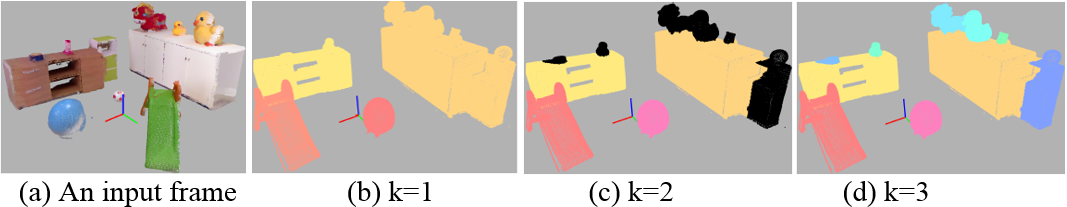
\includegraphics[width=2\columnwidth]{figures/object-iterations.png}
\caption{ The segmentation of each frame is progressively refined based on registered object models. From left to right: an input point cloud (a), segmentation updates at three iterations. \xj{show corresponding object model at each 
		iteration.} 	 }
\label{fig:object-iterations}
\end{figure*}
